\documentclass{beamer}

\usepackage[utf8]{inputenc} %cp1252 pour Windows, utf8 pour Linux
\usepackage[T1]{fontenc}
\usepackage{lmodern}
\usepackage{graphicx}
\usepackage[frenchb]{babel}
\usepackage{hyperref}

\usetheme{Warsaw}

\setbeamertemplate{blocks}[rounded]%
[shadow=true]

\title{Algorithme de \bsc{McNaughton} et \bsc{Yamada}}

\author{Elbert \bsc{Nyunting}\and Corentin \bsc{Chédotal} \and Ivan \bsc{Dromigny}}

\date{25 Janvier 2016}

\subject{Algorithme de \bsc{McNaughton} et \bsc{Yamada}}


\begin{document}

\begin{frame}
  \titlepage
\end{frame}

\begin{frame}{Table des matières}
  \tableofcontents
\end{frame}

\section{Introduction}
\begin{frame}{Introduction}{Auteurs}

   \uncover<2->{%
  \begin{block}{Robert \bsc{McNaughton} (1924--2014)}
        Mathématicien, logicien et informaticien théoricien.\\
        Pionnier de la théorie des automates et également auteur de contributions fondamentales en plusieurs domaines d'informatique théorique, comme langages formels, les grammaires et systèmes de réécriture ainsi que la combinatoire des mots.\\
        Il a plusieurs publications dont : \emph{Regular expressions and state graphs for automata}, en collaboration avec Hisao \bsc{Yamada}.
    \end{block}
    }
    
    \uncover<3->{%
    \begin{block}{Hisao \bsc{Yamada} (1930--2008)}
        Informaticien connu pour ses contributions importantes à l'informatique théorique et le développement des claviers japonais.
    \end{block}
    }

\end{frame}

\begin{frame}{Introduction}{L'algorithme}
   
    \uncover<2->{%
    \begin{block}{Brève description}
        Publié dans l'article \emph{Regular expressions and state graphs for automata} en 1960 par \bsc{McNaughton} et \bsc{Yamada}.\\
        Algorithme décrivant le passage d'un automate à état fini à l'expression rationnelle qui lui est associée.
    \end{block}
    }
    
    \uncover<3->{%
    \begin{exampleblock}{Nota}
        L'appellation "algorithme de \bsc{McNaughton} et \bsc{Yamada}" est parfois aussi utilisée pour parler d'un algorithme faisant le cheminement inverse (expression rationnelle vers automate $\varepsilon$-libre) décrit dans le même article.
    \end{exampleblock}
    }
    
\end{frame}

\section{Définitions essentielles}

\subsection{Expression rationnelle}

\begin{frame}{Expression rationnelle}

    Les expressions rationnelles sur $\Sigma$ décrivent les langages rationnels sur $\Sigma$. Elles sont définies ainsi :

    \uncover<2->{%
    \begin{alertblock}{Définition}
        \begin{itemize}
            \item L'expression rationnelle \O\ décrit le langage rationnel \O
            \item L'expression rationnelle $\varepsilon$ décrit le langage rationnel $\{\varepsilon\}$
            \item $\forall a \in \Sigma$, l'expression rationnelle $a$ décrit le langage rationnel $\{a\}$
            \item Soient $r_{1}$ et $r_{2}$, deux expressions rationnelles décrivant respectivement, les langages rationnels $L_{1}$ et $L_{2}$ sur $\Sigma$
            \begin{itemize}
                \item $r_{1} \union r_{2} = r_{1}|r_{2} = r_{1}+r_{2}$ décrit $L_{1} \union L_{2}$
                \item $r_{1} \cdot r_{2} = r_{1}r_{2}$ décrit $L_{1} \cdot L_{2}$
                \item $r_{1}^{*}$ décrit $L_{1}^{*}$
            \end{itemize}
        \end{itemize}
    \end{alertblock}
    }
    
\end{frame}

\subsection{Transition non-passante}

\begin{frame}{Transition non-passante}

    \uncover<2->{%
    \begin{alertblock}{Définition}
        Une transition non passante n'admet aucune dérivation. Elle est étiquetée \O. %vient du cours
    \end{alertblock}
    }
    
\end{frame}

\subsection{Automate généralisé}

\begin{frame}{Automate généralisé}{Définition du cours}

    \uncover<2->{%
    \begin{alertblock}{Définition}
        Un automate généralisé est un automate dont les transitions sont étiquetées par des expressions rationnelles.
    \end{alertblock}
    }
    
\end{frame}

\begin{frame}{Automate généralisé}{Détaillé}

    \uncover<2->{%
    \begin{block}{Plus en détails}
        \begin{itemize}
            \item L’état initial possède une transition vers tous les autres états (éventuellement une \emph{transition non passante})
            \item Aucun état n’a de transition vers l’état initial
            \item Il existe un et un seul état final
            \begin{itemize}
                \item distinct de l’état initial
                \item qui n’a aucune transition vers les autres états
                \item atteint par tous les autres états
            \end{itemize}
            \item Tous les états (sauf initial et final) possèdent une et une seule transition vers tous les autres états
        \end{itemize}
    \end{block}
    }
    
\end{frame}   

\section{L'algorithme de MacNaughton et Yamada}
\begin{frame}{L'algorithme de MacNaughton et Yamada}{Étape 0}
     \begin{columns}[T]
     \begin{column}{.48\textwidth}
        \indent Soit l’automate initial représenté par la la figure.
        \newline
        \newline
        \indent Pour rendre la figure plus lisible, nous allons représenter les arcs non passants $\emptyset$ par des traits pointillés.
     
     
     \end{column}
     
     \begin{column}{.48\textwidth}
     \begin{figure}
     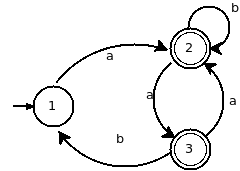
\includegraphics[scale=0.37]{Diagramme1.png}
     \centering
     \caption{Automate initial}     
     \end{figure}
     \end{column}
        
     \end{columns}

\end{frame}

\begin{frame}{L'algorithme de MacNaughton et Yamada}{Étape 1}
     \begin{columns}[T]
     \begin{column}{.48\textwidth}
         {\fontsize{8}{9}\selectfont Automate fini généralisé}
         \begin{itemize}
         
             \item {\fontsize{7}{8}\selectfont L'état initial possède une transition vers tous les autres états (éventuellement une transition $\emptyset$ );}
             \item {\fontsize{7}{8}\selectfont Aucun état a de transition vers l'état initial}

         \end{itemize}
     \end{column}
     
     \begin{column}{.48\textwidth}
     \begin{figure}
     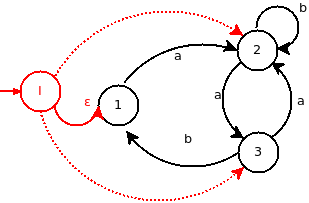
\includegraphics[scale=0.37]{Diagramme2_2.png}
     \centering
     \caption{Étape 1}     
     \end{figure}
     \end{column}
        
     \end{columns}

\end{frame}

\begin{frame}{L'algorithme de MacNaughton et Yamada}{Étape 1}
     \begin{columns}[T]
     \begin{column}{.48\textwidth}
         {\fontsize{8}{9}\selectfont Automate fini généralisé}
         \begin{itemize}
         
             \item {\fontsize{7}{8}\selectfont L'état initial possède une transition vers tous les autres états (éventuellement une transition $\emptyset$ );}
             \item {\fontsize{7}{8}\selectfont Aucun état a de transition vers l'état initial}
             \item {\fontsize{7}{8}\selectfont Il n'existe un et un seul état final distinct de l'état initial, sortant vers aucun autre état et atteignable par tous les autres états}

         \end{itemize}
     \end{column}
     
     \begin{column}{.48\textwidth}
     \begin{figure}
     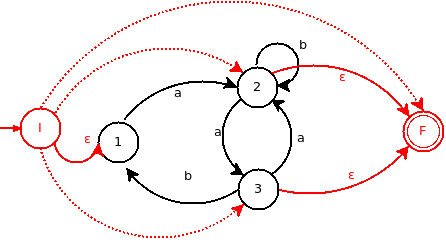
\includegraphics[scale=0.37]{Diagramme2_1.png}
     \centering
     \caption{Étape 1}     
     \end{figure}
     \end{column}
        
     \end{columns}

\end{frame}

\begin{frame}{L'algorithme de MacNaughton et Yamada}{Étape 1}
     \begin{columns}[T]
     \begin{column}{.48\textwidth}
         {\fontsize{8}{9}\selectfont Automate fini généralisé}
         \begin{itemize}
         
             \item {\fontsize{7}{8}\selectfont L'état initial possède une transition vers tous les autres états (éventuellement une transition $\emptyset$ );}
             \item {\fontsize{7}{8}\selectfont Aucun état a de transition vers l'état initial}
             \item {\fontsize{7}{8}\selectfont Il n'existe un et un seul état final distinct de l'état initial, sortant vers aucun autre état, atteignable par tous les autres états}
             \item
             {\fontsize{7}{8}\selectfont Tous les états (sauf initial et final) possèdent une \textbf{et une seule} transition vers tous les états. }
         \end{itemize}
     \end{column}
     
     \begin{column}{.48\textwidth}
     \begin{figure}
     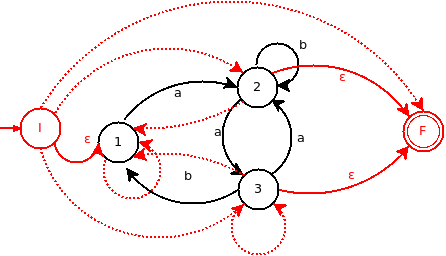
\includegraphics[scale=0.37]{Diagramme2.png}
     \centering
     \caption{Étape 1}     
     \end{figure}
     \end{column}
        
     \end{columns}

\end{frame}

\begin{frame}{L'algorithme de MacNaughton et Yamada}{Étape 2}
     \begin{columns}[T]
     \begin{column}{.48\textwidth}
         {\fontsize{8}{9}\selectfont Élimination d’un état ni initial ni final \textit{$q_e$}.}
         {\fontsize{8}{9}\selectfont La réduction consiste à éliminer \textbf{successivement} les états non initial et final.}
         \begin{itemize}
         
             \item {\fontsize{7}{8}\selectfont Nous allons enlever l'état 1 tout en gardant le langage.}
         \end{itemize}
     \end{column}
     
     \begin{column}{.48\textwidth}
     \begin{figure}
     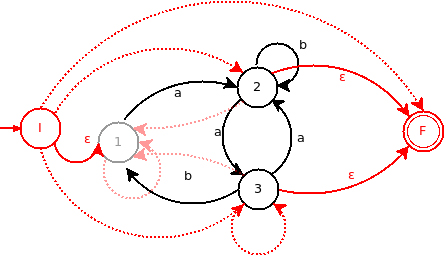
\includegraphics[scale=0.37]{Diagramme3_1.jpg}
     \centering
     \caption{Étape 2}     
     \end{figure}
     \end{column}
        
     \end{columns}   

\end{frame}

\begin{frame}{L'algorithme de MacNaughton et Yamada}{Étape 2}
     \begin{columns}[T]
     \begin{column}{.48\textwidth}
         {\fontsize{8}{9}\selectfont Élimination d’un état ni initial ni final \textit{$q_e$}.}
         {\fontsize{8}{9}\selectfont La réduction consiste à éliminer \textbf{successivement} les états non initial et final.}
         \begin{itemize}
         
             \item {\fontsize{7}{8}\selectfont Nous allons enlever l'état 1 tout en gardant le langage.}
             \item {\fontsize{7}{8}\selectfont Ici, \textit{I 1 2} est remplacé par la transition \textit{a} et donc \textit{I 2 3} est maintenant \textit{ab* a}.}
         \end{itemize}
     \end{column}
     
     \begin{column}{.48\textwidth}
     \begin{figure}
     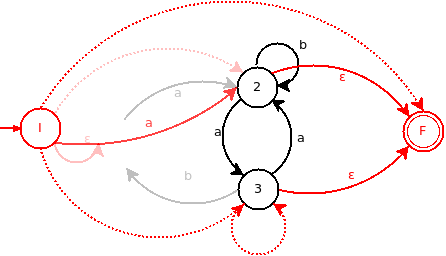
\includegraphics[scale=0.37]{Diagramme3_2.png}
     \centering
     \caption{Étape 2}     
     \end{figure}
     \end{column}
        
     \end{columns}   

\end{frame}

\begin{frame}{L'algorithme de MacNaughton et Yamada}{Étape 2}
     \begin{columns}[T]
     \begin{column}{.48\textwidth}
         {\fontsize{8}{9}\selectfont Élimination d’un état ni initial ni final \textit{$q_e$}.}
         {\fontsize{8}{9}\selectfont La réduction consiste à éliminer \textbf{successivement} les états non initial et final.}
         \begin{itemize}
         
             \item {\fontsize{7}{8}\selectfont Nous allons enlever l'état 1 tout en gardant le langage.}
             \item {\fontsize{7}{8}\selectfont Ici, \textit{I 1 2} est remplacé par la transition \textit{a} et donc \textit{I 2 3} est maintenant \textit{ab* a}.}
             \item {\fontsize{7}{8}\selectfont Ensuite \textit{3 2 3} aura comme transition \textit{(ba|a)b* a}}
         \end{itemize}
     \end{column}
     
     \begin{column}{.48\textwidth}
     \begin{figure}
     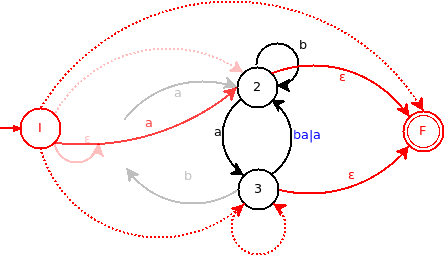
\includegraphics[scale=0.37]{Diagramme3_3.png}
     \centering
     \caption{Étape 2}     
     \end{figure}
     \end{column}
        
     \end{columns}   

\end{frame}


\begin{frame}{L'Algorithme de MacNaughton et Yamada}{Etape 3}
     \begin{columns}[T]
     \begin{column}{.48\textwidth}
         {\fontsize{8}{9}\selectfont Élimination de l'état 2.}       
         \begin{itemize}
         
             \item {\fontsize{7}{8}\selectfont Maintenant débarrassons nous de l'état 2.}
             
         \end{itemize}
     \end{column}
     
     \begin{column}{.48\textwidth}
     \begin{figure}
     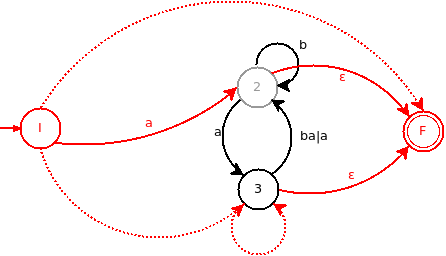
\includegraphics[scale=0.37]{Diagramme4_1.png}
     \centering
     \caption{Étape 3}     
     \end{figure}
     \end{column}
        
     \end{columns}
\end{frame}

\begin{frame}{L'Algorithme de MacNaughton et Yamada}{Etape 3}
     \begin{columns}[T]
     \begin{column}{.48\textwidth}
         {\fontsize{8}{9}\selectfont Élimination de l'état 2.}
         \begin{itemize}
         
             \item {\fontsize{7}{8}\selectfont Maintenant débarrassons nous de l'état 2.}
             \item {\fontsize{7}{8}\selectfont Nous avons donc \textit{I F} qui remplace \textit{I 2 F} avec comme transition \textit{ab*} et qui "concrétise" la transition $\emptyset$ partant de I vers F}
             
         \end{itemize}
     \end{column}
     
     \begin{column}{.48\textwidth}
     \begin{figure}
     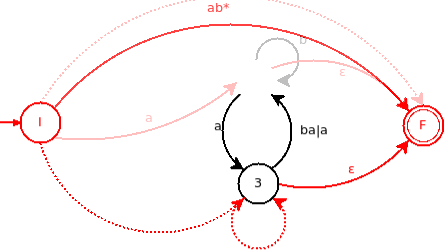
\includegraphics[scale=0.37]{Diagramme4_2.png}
     \centering
     \caption{Étape 3}     
     \end{figure}
     \end{column}
        
     \end{columns}
\end{frame}

\begin{frame}{L'Algorithme de MacNaughton et Yamada}{Etape 3}
     \begin{columns}[T]
     \begin{column}{.48\textwidth}
         {\fontsize{8}{9}\selectfont Élimination de l'état 2.}
         \begin{itemize}
         
             \item {\fontsize{7}{8}\selectfont Maintenant débarrassons nous de l'état 2.}
             \item {\fontsize{7}{8}\selectfont Nous avons donc \textit{I F} qui remplace \textit{I 2 F} avec comme transition \textit{ab*} et qui "concrétise" la transition $\emptyset$ partant de I vers F}
             \item {\fontsize{7}{8}\selectfont La voie \textit{I 2 3}, qui était \textit{ab* a} passe directement de \textit{I} à \textit{3} par la transition \textit{ab* a}}
             
         \end{itemize}
     \end{column}
     
     \begin{column}{.48\textwidth}
     \begin{figure}
     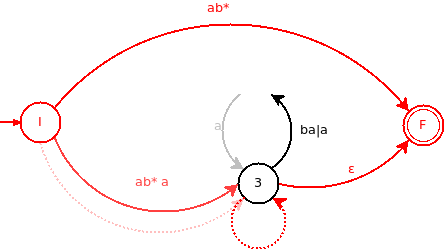
\includegraphics[scale=0.37]{Diagramme4_3.png}
     \centering
     \caption{Étape 3}     
     \end{figure}
     \end{column}
        
     \end{columns}
\end{frame}

\begin{frame}{L'Algorithme de MacNaughton et Yamada}{Etape 3}
     \begin{columns}[T]
     \begin{column}{.48\textwidth}
         {\fontsize{8}{9}\selectfont Élimination de l'état 2.}
         \begin{itemize}
         
             \item {\fontsize{7}{8}\selectfont Maintenant débarrassons nous de l'état 2}
             \item {\fontsize{7}{8}\selectfont Nous avons donc \textit{I F} qui remplace \textit{I 2 F} avec comme transition \textit{ab*} et qui "concrétise" la transition $\emptyset$ partant de I vers F}
             \item {\fontsize{7}{8}\selectfont La voie \textit{I 2 3}, qui était \textit{ab* a} passe directement de \textit{I} à \textit{3} par la transition \textit{ab* a}}
             \item {\fontsize{7}{8}\selectfont De même, la boucle sur 3 est maintenant \textit{(ba|a)b* a}}
             
         \end{itemize}
     \end{column}
     
     \begin{column}{.48\textwidth}
     \begin{figure}
     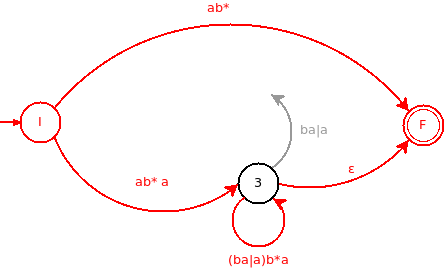
\includegraphics[scale=0.37]{Diagramme4_4.png}
     \centering
     \caption{Étape 3}     
     \end{figure}
     \end{column}
        
     \end{columns}
\end{frame}

\begin{frame}{L'Algorithme de MacNaughton et Yamada}{Etape 3}
     \begin{columns}[T]
     \begin{column}{.48\textwidth}
         {\fontsize{8}{9}\selectfont Élimination de l'état 2.}
         \begin{itemize}
         
             \item {\fontsize{7}{8}\selectfont Maintenant débarrassons nous de l'état 2}
             \item {\fontsize{7}{8}\selectfont Nous avons donc \textit{I F} qui remplace \textit{I 2 F} avec \textit{ab*}, la transition $\emptyset$ partant de I vers F}
             \item {\fontsize{7}{8}\selectfont La voie \textit{I 2 3}, qui était \textit{ab* a} passe directement de \textit{I} à \textit{3} par la transition \textit{ab* a}}
             \item {\fontsize{7}{8}\selectfont De même, la boucle sur 3 est maintenant \textit{(ba|a)b* a}}
             \item {\fontsize{7}{8}\selectfont Et enfin, \textit{I 3 F} est maintenant \textit{(ba|a)b*|$\epsilon$}}
             
         \end{itemize}
     \end{column}
     
     \begin{column}{.48\textwidth}
     \begin{figure}
     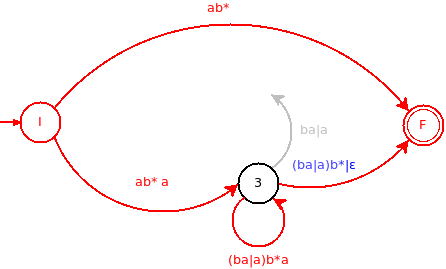
\includegraphics[scale=0.37]{Diagramme4_5.png}
     \centering
     \caption{Étape 3}     
     \end{figure}
     \end{column}
        
     \end{columns}
\end{frame}

\begin{frame}{L'Algorithme de MacNaughton et Yamada}{Fin}
        \begin{columns}[T]
     \begin{column}{.48\textwidth}
         {\fontsize{8}{9}\selectfont Élimination de l'état 3.}
         \begin{itemize}
         
             \item {\fontsize{7}{8}\selectfont Pour terminer, nous allons éliminer l'état 3}
             
             
         \end{itemize}
     \end{column}
     
     \begin{column}{.48\textwidth}
     \begin{figure}
     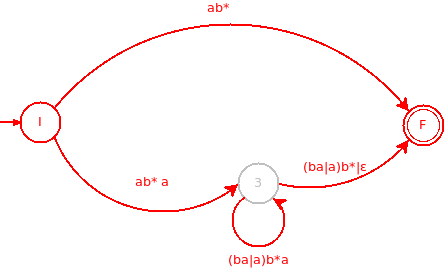
\includegraphics[scale=0.37]{Diagramme5_1.png}
     \centering
     \caption{Fin}     
     \end{figure}
     \end{column}
        
     \end{columns}
\end{frame}

\begin{frame}{L'Algorithme de MacNaughton et Yamada}{Fin}
        \begin{columns}[T]
     \begin{column}{.48\textwidth}
         {\fontsize{8}{9}\selectfont Élimination de l'état 3.}
         \begin{itemize}
         
             \item {\fontsize{7}{8}\selectfont Pour terminer, nous allons éliminer l'état 3}
             \item {\fontsize{7}{8}\selectfont \textit{I F} aura donc comme transition \textit{ab*a((ba|a)b*a)* ((ba|a)b*|$\epsilon$)}  }
             
             
         \end{itemize}
     \end{column}
     
     \begin{column}{.48\textwidth}
     \begin{figure}
     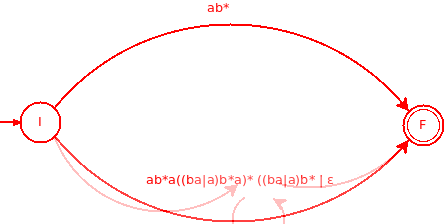
\includegraphics[scale=0.37]{Diagramme5_2.png}
     \centering
     \caption{Fin}     
     \end{figure}
     \end{column}
        
     \end{columns}
\end{frame}

\begin{frame}{L'Algorithme de MacNaughton et Yamada}{Fin}
        \begin{columns}[T]
     \begin{column}{.48\textwidth}
         {\fontsize{8}{9}\selectfont Élimination de l'état 3.}
         \begin{itemize}
         
             \item {\fontsize{7}{8}\selectfont Pour terminer, nous allons éliminer l'état 3}
             \item {\fontsize{7}{8}\selectfont \textit{I F} aura donc comme transition \textit{ab*a((ba|a)b*a)* ((ba|a)b*|$\epsilon$)}  }
             \item {\fontsize{7}{8}\selectfont L'expression résultant est donc \big{(}ab*a((ba|a)b*a)* ((ba|a)b*|$\epsilon$)\big{)} | ab*} 
             
             
         \end{itemize}
     \end{column}
     
     \begin{column}{.48\textwidth}
     \begin{figure}
     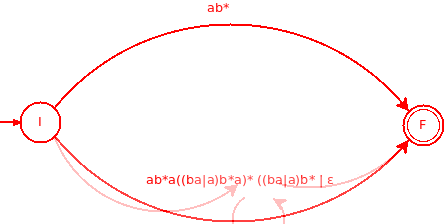
\includegraphics[scale=0.37]{Diagramme5_2.png}
     \centering
     \caption{Fin}     
     \end{figure}
     \end{column}
        
     \end{columns}
\end{frame}

    


\section{Références}
\begin{frame}{Références bibliographiques}
    \uncover<2->{%
    \begin{block}{Livres}
        \begin{itemize}
            \item \bsc{Wolper}, Pierre. \emph{Introduction à la calculabilité.} 2006 -- Disponible à la BU
        \end{itemize} 
    \end{block}
     }
     
    \uncover<3->{%
    \begin{block}{Cours}
        \begin{itemize}
            \item \bsc{Amsili}, Pascal. \href{http://www.linguist.univ-paris-diderot.fr/~amsili/Perm/polyLangagesRationnels_2014_1.10.pdf}{\emph{Langages rationnels.}} Université Paris Diderot : Master de Linguistique Informatique. Février 2014 -- Disponible en ligne, consulté le 23 Janvier 2016
            \item \bsc{Enguehard}, Chantal et \bsc{Monfroy} Eric. \emph{X6I0020 -- Fondements de calculs et de calculabilité.} Université de Nantes : Licence 3 Informatique. 2016/2017 -- Disponible sur Madoc, consulté le 23 Janvier 2016

        \end{itemize} 
    \end{block}
    }   
    
\end{frame}

\end{document}

